%955
\newpage
\section{プログラムと\ruby{画像}{が|ぞう}ファイルについて知ろう}


\subsection{絵を出してみよう}


ゲームを作る場合には、きれいな絵を出したいですよね。

ここでは、HSPで文字だけでなく、絵を出す方法について学んでいきましょう。

\bigskip

まずは、簡単なプログラムから見てみましょう。

スクリプトエディタの、ファイル→「開く」メニューから「celput.hsp」を読み込んでください。

終わったら、さっそく[F5]キーを押してプログラムを実行してみましょう。


\begin{figure}[H]
    \begin{center}
      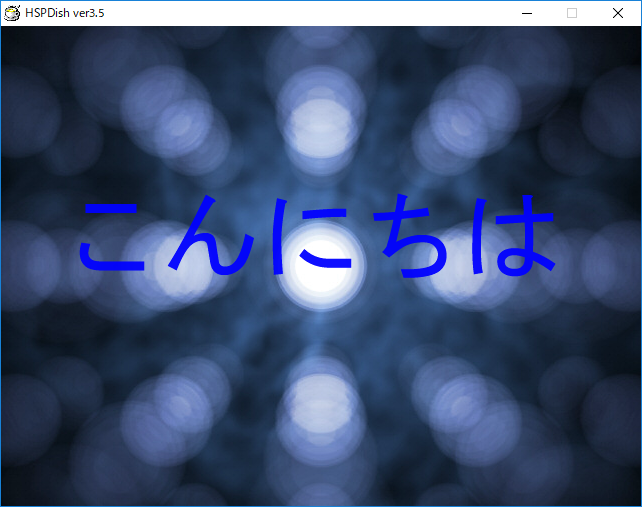
\includegraphics[keepaspectratio,width=10.028cm,height=7.909cm]{text04-img/text04-img012.png}
      \caption{celput.hspの実行画面}
    \end{center}
    \label{fig:prog_menu}
\end{figure}


今度は、\ruby{背景}{はい|けい}に絵が出ました。

この絵は、あらかじめ「sozai1.jpg」というファイルで\ruby{用意}{よう|い}されているものです。

実際に絵を出すためには、画像ファイルと呼ばれる絵のデータが必要になります。

それが、「sozai1.jpg」になります。(画像ファイルは、GIMPツールや、ブラウザなどで開くことができます。)


絵を出すためには、2つの命令を使う必要があります。1つ目のcelloadは、必要な絵の素材を知らせるための命令です。これにより、指定された素材を表示する準備をします。

\begin{description}
    \item \textgt{\bf \ \ celload “画像ファイル名” , 絵の番号\ \ \ \ \texttt{← 絵を出す準備をする}}
\end{description}


一度、celload命令によって\ruby{登録}{とう|ろく}された絵は、celput命令によって表示させることができます。

celload命令は、最初の1回だけ実行すれば良いです。以降は、celput命令によって、mes命令やboxf命令と同じように絵を出すことができるようになります。


celput命令は、以下のように書くことができます。




\begin{description}
    \item \textgt{\bf celput 絵の番号}
\end{description}



絵の番号というのは、celload命令で指定していた番号のことです。

出すための絵を登録する時に、1,2,3,4…というように、別々な番号を\ruby{割}{わ}り\ruby{振}{ふ}っておいて、同時に色々な絵を出せるようにするための仕組みです。

最初は、番号1を使っておきましょう。


\begin{figure}[H]
    \begin{center}
      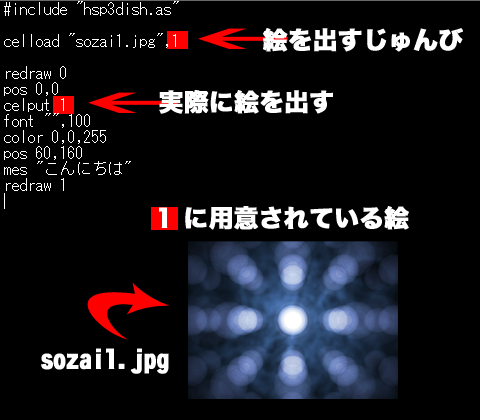
\includegraphics[keepaspectratio,width=12.806cm,height=11.206cm]{text04-img/text04-img013.png}
    \end{center}
    \label{fig:prog_menu}
\end{figure}


つまり、


\begin{description}
    \item \textgt{\bf \ \ celload “sozai1.jpg”,1}
\end{description}

は、番号1で「sozai1.jpg」の絵を表示するための準備をするという意味になります。

celputで指定した番号に準備された絵を表示します。

表示する位置は、mes命令などと同じようにpos命令で指定された位置になります。

準備する画像のファイルは、プログラム(.hsp)がある場所と同じフォルダに入れておく必要があります。

画像ファイル、「sozai1.jpg」は、04フォルダ内にあるはずです。


celload命令とcelput命令、絵を出す番号と画像ファイルの\ruby{関係}{かん|けい}をよく覚えておきましょう。

\newpage
\subsection{例題に挑戦しよう}


終わってしまった人は、以下の例題にも挑戦してみよう。


・色々な絵と文字を表示しよう

・自分で用意した絵を表示する

例題の考え方がわからない時は、近くのTAか先生に聞いてください。

わからない所は、そのままにせず、必ず答えを見つけてから先に進みましょう。













